%%%%%%%%%%%%%%%%%%%%%%%%%%%%%%%%%
%%%%%%%%%%%% CHAPTER %%%%%%%%%%%%
%%%%%%%%%%%%%%%%%%%%%%%%%%%%%%%%%
\chapter{Methods}

\section{Data simulation}
\label{sec:data simulation}
\subsection{Cosmology}
\label{subsec:cosmology}

\begin{wraptable}{r}{2.8cm}
%\vspace{-0.7cm}
\centering
\caption{\label{tab:fiducial_cosmology}Fiducial cosmology values given to \code{jaxcosmo}.}
%% Given these simple cosmological parameters, $S_8=\sigma_8\sqrt{\Omega_m/0.3}$ will take the value of $0.8$.
  \begin{tabular}{ll}
    \toprule
     & Fiducial \\
    \midrule
    $\Omega_m$ & 0.3 \\
    $\Omega_b$ & 0.05 \\
    $\Omega_k$ & 0 \\
    $h$ & 0.7 \\
    $n_s$ & 0.97 \\
    $\sigma_8$ & 0.8 \\
    $w_0$ & -1 \\
    $w_a$ & 0 \\
    \bottomrule
  \end{tabular}
\end{wraptable} 
This work follows in the general footsteps of data analysis of weak lensing surveys like \textit{HSC} \cite{cosmology:hsc} and \textit{KiDS} \cite{cosmology:kids450}\cite{cosmology:kids1000}, as we aim to replicate their methodologies.
Throughout the work, we assume a fiducial cosmology of fixed parameter values as shown in \textit{Tab. }\ref{tab:fiducial_cosmology}. In particular, all data maps will be generated from a power spectrum following this cosmology. We will refer to this power spectrum as the fiducial power spectrum $C(l)$. A leading modelling choice comes with the redshift distribution $n(z)$. We model it as a Smail-type distribution \cite{smail}\cite{smail2},
\begin{equation}
    n(z)=z^\alpha \exp{\left[-\left(\frac{z}{z_0}\right)^\beta\right]}.
\end{equation}
The choice of parameters has been made to emulate bin 5 of the \textit{KiDS1000} survey \cite{cosmology:kids1000_bins}, with parameters $\alpha=3.5$, $\beta=4.5$, $z_0=1$. 

\begin{figure}[h]
    \centering
    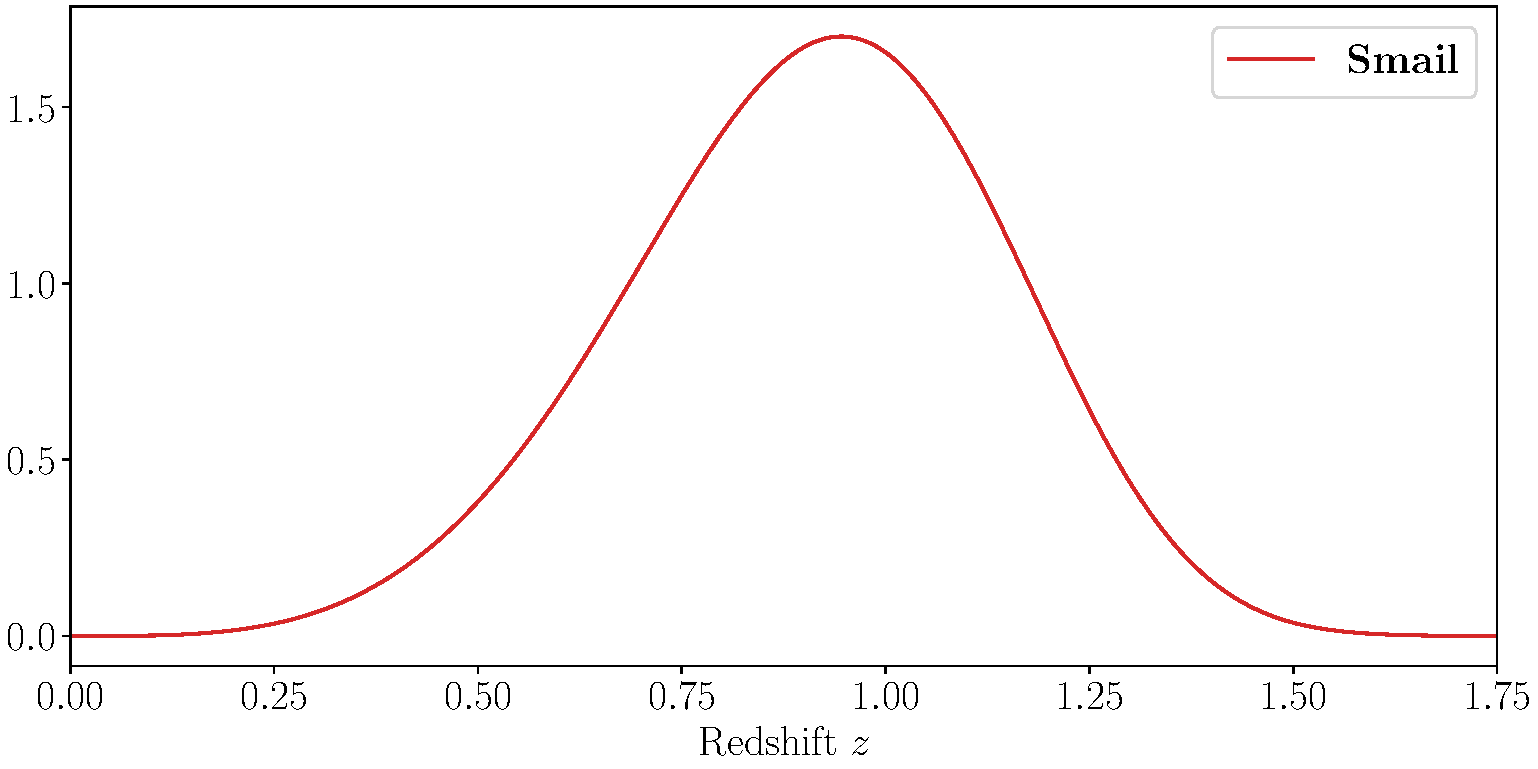
\includegraphics[width=\textwidth]{images/2_smail.pdf}
    \captionof{figure}{Smail-type redshift distribution for the chosen parameters: $\alpha=3.5$, $\beta=4.5$, $z_0=1$.}
    \label{fig:smail}
\end{figure}

\begin{comment}
"Omega_m": 0.3,
"Omega_b": 0.05,
"Omega_k": 0.0,
"h": 0.7,
"n_s": 0.97,
"S8": 0.8,
"w0": -1.0,
"wa": 0.0, 
\end{comment}

\subsection{Map making pipeline}
\label{sec:map making pipeline}
When dealing with maps of finite size $(L, L)$ and pixel resolution $(N,N)$, Fourier space is going to have boundaries, just as real space does. These limits are given by
\begin{gather*}
    l_{\text{min}} = \frac{2\pi}{L},\\
    l_{\text{max}} = \frac{2\pi}{L} N.
\end{gather*}
Therefore, a map of size $(10^{\circ},10^{\circ})$ and a grid $64\times64$ will have limits $(l_{\text{min}}, l_{\text{max}}) = (36, 2304)\text{rad}^{-1}$. Now that we have the physical range for the power spectrum, we can generate data.
\begin{figure}[h]
%\centering
\begin{tikzpicture}[>=stealth, node distance=2.5cm]
  % Nodes
  \node[diamond, draw=black, fill=black, text=white, minimum size=18mm, font=\Large, rounded corners] (a) at (0,0) {$C(l)$};
  \node[diamond, draw=black, fill=white, minimum size=18mm, font=\Large, rounded corners] (b) at (1.5,1.5) {$\tilde{w}^{L}$};
  \node[diamond, draw=black, fill=white, minimum size=18mm, font=\Large, rounded corners] (c) at (4,1.5) {$\tilde{w}^{G}$};
  \node[diamond, draw=black, fill=white, minimum size=18mm, font=\Large, rounded corners] (d) at (6.5,1.5) {$\tilde{C}^{G}$};
  \node[circle, draw=black, fill=white, text=black, minimum size=14mm, font=\Large, rounded corners] (e) at (8.9,1.5) {$\tilde{\kappa}^{G}$};
  \node[circle, draw=black, fill=black, text=white, minimum size=14mm, font=\Large, rounded corners] (f) at (11,1.5) {$\kappa^{L}$};
  \coordinate (g) at (1.3,-1.5);
  \node[circle, draw=black, fill=black, text=white, minimum size=14mm, font=\Large, rounded corners] (h) at (11,-1.5) {$\kappa^{G}$};

  % Arrows
  \draw[->, line width=1.5pt] (a) to[out=90, in=180, looseness=1.2] node[near end, above] {$\mathcal{H}^{-1}$} (b);
  \draw[-, line width=1.5pt] (a) to[out=270, in=180, looseness=1.2] (g);
  \draw[->, line width=1.5pt] (g) -- node[above] {\textit{GRF}} (h);
  \draw[->, line width=1.5pt] (e) -- node[above] {$\mathcal{L}_\kappa$} (f);
  \draw[->, line width=1.5pt] (b) -- node[above] {$\mathcal{L}_w^{-1}$} (c);
  \draw[->, line width=1.5pt] (c) -- node[above] {$\mathcal{H}$} (d);
  \draw[->, line width=1.5pt] (d) -- node[above] {\textit{GRF}} (e);
\end{tikzpicture}

\caption{Sequence of transformations used to generate Gaussian and lognormal maps starting from the fiducial angular power spectrum. The top branch shows how to generate a GRF which when transformed to a lognormal field, follows the fiducial $C(l)$.  The bottom branch is a standard GRF realisation starting from the fiducial $C(l)$. $L$ and $G$ stand for lognormal and Gaussian respectively. $\mathcal{H}$ is the Hankel transformation, and tilde refers to intermediate results.}
\label{tik:cw}
\end{figure}

To generate a GRF, we employ the algorithm mentioned in \textit{Eq. }\eqref{eq:grf 2D}. However, in making a lognormal field, the matter is a bit more complicated. Any GRF on which we apply the lognormal transformation $\mathcal{L}_\kappa$, from \textit{Eq. }\eqref{eq:L_k}, becomes a lognormal field. The reason we do not just lognormal transform any field is given by the fact that they would not recover the fiducial power spectrum $C(l)$. Our goal is therefore to find a transfer GRF $\tilde{\kappa}^G$ which, when transformed lognormally, gives rise to a lognormal field $\kappa^L$ that recovers $C(l)$. To do so, we follow the sequence of transformations illustrated in the top branch of \textit{Fig. }\ref{tik:cw}.

\subsection{Noise and mask}
\begin{figure}[h]
    \centering
    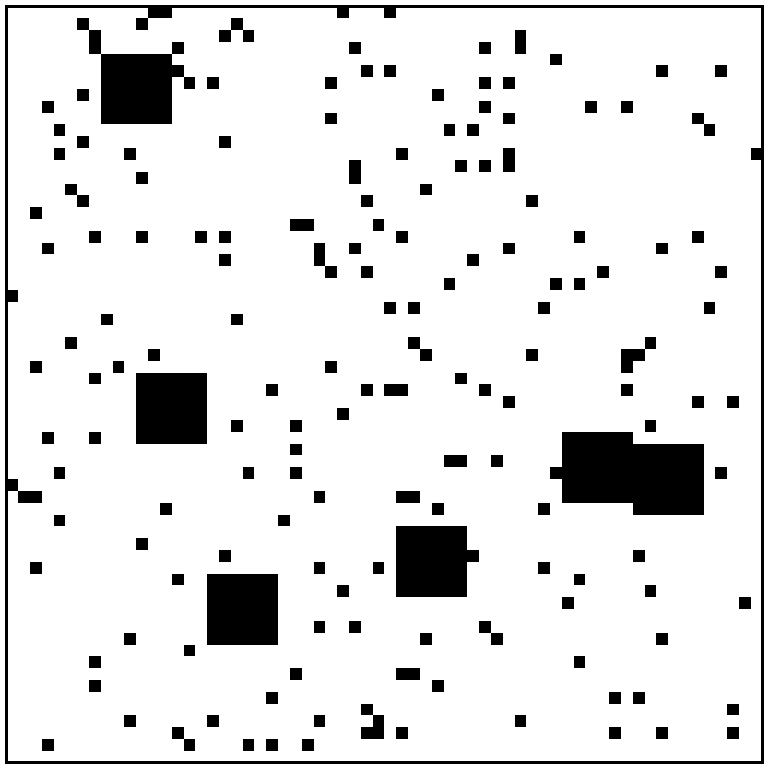
\includegraphics[width=0.5\linewidth]{images/5_random_and_blocks_mask.pdf}
    \caption{Approximately $10\%$ mask applied to the data. Size $(10^{\circ},10^{\circ})$ and grid $64\times64$.}
    \label{fig:mask}
\end{figure}
As all data is being simulated, we only take into account the so-called shape noise, which is due to the intrinsic distribution of ellipticities and angle formed with respect to us. GPs will treat each pixel of the map as a random variable Gaussianly distributed with standard deviation given by \cite{noise},
\begin{equation}
    \sigma_\text{noise} = \frac{\sigma_e}{\sqrt{n_g A_{px}}}.
    \label{eq:noise}
\end{equation}
We use values of $\sigma_e=0.26$, $n_g= 4, 10, 30, 100 \text{ galaxies}/\text{arcmin}^2$, and a pixel area given by the pixel resolution squared, $A_{px}=(L/N)^2$. For our highest-resolution run, we have $N=64$ and use $n_g = 10 \text{ galaxies}/\text{arcmin}^2$, which results in a noise standard deviation of $\sigma_\text{noise} \sim 0.0088$. The mask being used as seen in \textit{Fig. }\ref{fig:mask}, covers approximately $10\%$ of the patch \cite{pixel}. We keep the noise and mask random seeds fixed throughout the work.

\section{Kernel}
\label{sec:gaussian process kernel}
The kernel of a Gaussian process is given by a function of the form $k(x,y)$. It takes in two points, $x$ and $y$, and returns the value of their correlation. In our case, specifically, $x$ and $y$ will be two points in a grid of shape $(N,N)$, and the kernel function will be the convergence angular autocorrelation function. As all code used for this paper is written in \code{JAX} \cite{jax} we opt for the use of the library \code{tinygp} \cite{tinygp} for all Gaussian process computations. \code{tinygp} allows for the use of a custom kernel with a custom \code{evaluate} method, which takes two points on the grid and returns the correlation value. We follow with two \code{Python} pseudocodes of our kernel implementations.
\begin{lstlisting}[language=Python, label={lst:hankel}, caption=\code{kernel_Hankel} uses the helper function \code{Hankel} which returns a 1D callable correlation function \code{w}. Then finds the euclidean distance between $x$ and $y$ and evaluates the correlation function at that point. We will discuss how we perform the Hankel transformation in the following section.]
class kernel_Hankel:
    def __init__(self, cl, N, L):
        self.w   = Hankel(cl, N, L)
        self.r   = L / N
        
    def evaluate(self, x, y):
        theta    = self.r * sqrt(sum(x - y))
        return self.w(theta)
\end{lstlisting}
 
\begin{lstlisting}[language=Python, label={lst:FFT}, caption=\code{kernel_FFT} performs a 2D Fourier transform on the power spectrum \code{cl2D}. This returns a 2D array that is the correlation function. Then to evaluate \code{w2D} we need two indices. These are given by the difference of $x$ and $y$ component wise. Furthermore we have to be careful about possible mismatches between the shape of \code{cl2D} and the grid of our map. For this we have the renormalisation factor \code{r}. We will discuss further how we get \code{cl2D} in the following section.]
class kernel_FFT:
    def __init__(self, cl2D, N, L):
        M        = sqrt(cl2D.size)
        self.w2D = abs(ifft2(cl2D)) * M**2 / L**2
        self.r   = M / N
        
    def evaluate(self, x, y):
        d0       = self.r * abs(x[0] - y[0])
        d1       = self.r * abs(x[1] - y[1])
        return self.w2D[int(d0)][int(d1)]
\end{lstlisting}

\subsection{Hankel transform}
\label{sec:Hankel transform}
In order to build a Gaussian process kernel, we need to find the correlation function that best describes the data. The way we do this is by computing the angular power spectrum and transforming it in the corresponding angular correlation function. Let's explore the previously discussed flat-sky relation between angular power spectrum and correlation function given by \textit{Eq. }\eqref{eq:flatsky hankel}. This particular integral of a Bessel function is also known as a zeroth order Hankel transformation,
\begin{equation}
    w(\theta) = \int \frac{dl}{2\pi} l C(l) J_0(l\theta).
    \label{eq:C-w hankel}
\end{equation}
We will explore two methods for computing this integral: the \textit{integration} method \textit{Sec. }\ref{sec:integration method} and the \textit{FFTlog} method \textit{Sec. }\ref{sec:FFTlog method}.

\subsubsection{Integration}
\label{sec:integration method}
Integration is the most straight forward way to evaluate the integral, but it requires to implement an algorithm for the approximation of the Bessel function $J_0$. The advantages of this method:
\begin{itemize}
    \item it is easy to integrate over the correct $l$-range, from $l_{\text{min}}$ and $l_{\text{max}}$, a freedom that we do not have with the FFTlog.
\end{itemize}
The disadvantages:
\begin{itemize}
    \item integration is computationally slow, especially when dealing with highly oscillatory behaviour introduced by the Bessel function, which requires fine sampling.
\end{itemize}

\subsubsection{FFTlog}
\label{sec:FFTlog method}
The FFTlog method \cite{fftlog} is a fast implementation of the Hankel transformation. In fact it simplifies \textit{Eq. }\eqref{eq:C-w hankel} by assuming a power decomposition of $C(l)$. Such a decomposition is achievable by taking the \textit{fast Fourier transformation (FFT)} in $\log k$, hence the name FFTlog. The power spectrum becomes,
\begin{equation}
    C(l)=\sum_\alpha c_\alpha l^{\upsilon + i\eta_\alpha}.
\end{equation}
Substituting in \textit{Eq. }\eqref{eq:C-w hankel},
\begin{equation*}
    w(\theta) = \sum_\alpha c_\alpha \int_0^\infty \frac{dl}{2\pi} l^{\upsilon + i\eta_\alpha+1} J_0(l\theta).
\end{equation*}
Take $x=l\theta$ and $s_\alpha-1=\upsilon + i\eta_\alpha+1$,
\begin{equation*}
    w(\theta) = \sum_\alpha c_\alpha \theta^{-s_\alpha} \int_0^\infty \frac{dx}{2\pi} x^{s_\alpha-1} J_0(x).
\end{equation*}
Lastly we recognise $\int_0^\infty dx x^{s-1}J_0(x) = \frac{2^{s-1}}{\pi}\sin(\pi s/2) [\Gamma(s/2)]^2$, a Mellin transform. Using this tabulated result we conclude that the correlation is given by the sum,
\begin{equation}
    w(\theta) = \frac{1}{2\pi^2}\sum_\alpha c_\alpha \theta^{-s_\alpha}2^{s_\alpha-1}\sin(\pi s_\alpha/2) [\Gamma(s_\alpha/2)]^2.
\end{equation}
For the Mellin transform identity to hold analytically, the integral bounds have to go from 0 to $\infty$. Although computationally we don't need to consider such a wide range, we still have to broaden the integration limits to something larger than our $l$-range; so as to avoid ringing effects. Experimentally we have found that extending the $l$-range between $l_{\text{min}}/4$ and $l_{\text{max}}$, is enough to compensate for such effects. The advantages of this method:
\begin{itemize}
    \item the FFTlog method is ultimately much faster than the integration method.
\end{itemize}
The disadvantages:
\begin{itemize}
    \item the widening of the $l$-range needed to avoid ringing effects inevitably adds power to the correlation function resulting in a higher variance and overall amplitude.
\end{itemize}

\subsection{Fourier transform}
The second transformation that we can use to go from power spectrum to correlation function, is the Fourier transformation discussed in \textit{Eq. }\eqref{eq:flatsky fft}. It is a more fundamental relation than the Hankel transformation as it does not assume that $l$ is radially symmetric. In our case, low resolution, coupled with a square map, means that the radial assumption might not apply. Note that, the lowest resolution grid we use is $32\times32$, with $L/N \sim 19$ arcmin; which is one order of magnitude worse than today's weak lensing data, around $\sim 3$ arcmin according to \cite{fwdmodel}.  In the following \textit{Sec. }\ref{sec:gaussian process kernel} we will find experimentally that the Hankel methods described above do not work well with our GP setup. For this reason, we explore this method of conversion between angular power spectrum and correlation function,
\begin{equation}
    w(\theta)=\int\frac{d^2l}{4\pi^2}e^{-i\bm{l}\cdot\bm{\theta}}C(l).
    \label{eq:C-w fft}
\end{equation}
As computers can only deal with discrete functions, it is important to note that we will be performing a \textit{discrete Fourier transformation (DFT)}. We will use the widely known FFT algorithm to compute DFTs. In particular we use JAX's implementation of the 2D FFT algorithm, \code{jax.numpy.fft.ifft2}. 

Let us find the relation between continuous Fourier transformation and DFT. The definitions of continuous and discrete Fourier transformations in 1D, are respectively:
\begin{align} 
    \mathcal{F}^{-1}&=\int\frac{dk}{2\pi}e^{ikx}, \label{eq:F}\\
    \text{F}^{-1}&=\frac{1}{N}\sum_p e^{ik_px}. \label{eq:DFT}
\end{align}
First of all, a DFT is dimensionless. Secondly, it is discrete and bounded. We can therefore rewrite \textit{Eq. }\eqref{eq:F} using the substitution $k(p)=2\pi \frac{p}{L}$ to discretise k-space,
\begin{equation*}
     \int\frac{dk}{2\pi}e^{ikx} = \int\frac{dp}{L} e^{ik(p)x} = \frac{1}{L}\sum_p e^{ik_px}.
\end{equation*}
Applying the definition of DFT as seen in \textit{Eq. }\eqref{eq:DFT}, it follows that in 1D
\begin{equation}
    \mathcal{F}^{-1}=\frac{N}{L}\text{F}^{-1}.
\end{equation}
Which means that the correlation function is given by a \textit{backwards} normalised inverse DFT to be scaled by a factor $(N/L)^d$, where $d$ is the dimension of the considered space. In our case, $d=2$. 

In order to perform a FFT in 2D, we will need a two dimensional extension of the angular power spectrum. We make use of its radial symmetry with respect to $\bm{l}=(l_x,l_y)$ and create a 2D grid of shape $(M,M)$ as shown in \textit{Fig. }\ref{tik:1D to 2D}. 
\begin{figure}[h]
\centering
\begin{tikzpicture}
  % Nodes
  \node[diamond, draw=black, fill=black, text=white, minimum size=18mm, font=\Large, rounded corners] (a) at (0,0) {$C^{1D}$};
  \node[diamond, draw=black, fill=black, text=white, minimum size=18mm, font=\Large, rounded corners] (b) at (5,0) {$C^{2D}$};

  % Arrows
  \draw[->, line width=1.5pt] (a) -- node[above] {$l \equiv \sqrt{l_x^2+l_y^2}$} (b);
\end{tikzpicture}
\caption{1D to 2D extension of the power spectrum $C(l)$}
\label{tik:1D to 2D}
\end{figure}
Now that we have a 2D power spectrum we can take the inverse two dimensional fast Fourier transformation to obtain a 2D correlation function. In practice, we will test two grids, which we name \textit{full-range FFT} method and \textit{half-range FFT} method. 
\subsubsection{Full-range FFT}
The full-range FFT is defined by a grid of shape $(2N,2N)$. Since the grid is radial, it will be centered. This implies that if we want to keep information of all $N$ modes,
\begin{equation}
    \frac{2\pi}{L},\, \frac{4\pi}{L},\,\cdot\cdot\cdot\,,\, \frac{2\pi}{L}N,
\end{equation}
the grid will have to be at least of shape $M=2N$.
The advantages of this method:
\begin{itemize}
    \item it keeps information on the full range of modes.
\end{itemize}
The disadvantages:
\begin{itemize}
    \item it introduces rounding errors, as the field has shape $(N,N)$ and not all of the possible distance combinations of such a grid are covered bya grid of shape $(2N,2N)$.
\end{itemize}
\subsubsection{Half-range FFT}
The half-range FFT is defined by a grid of shape $(N,N)$.
The advantages of this method:
\begin{itemize}
    \item has the perk of having no shape mismatch between field and correlation function.
\end{itemize}
The disadvantages:
\begin{itemize}
    \item it loses half of the $l$-range, missing information on small scales.
\end{itemize}